% Options for packages loaded elsewhere
\PassOptionsToPackage{unicode}{hyperref}
\PassOptionsToPackage{hyphens}{url}
%
\documentclass[
  9pt,
  ignorenonframetext,
]{beamer}
\usepackage{pgfpages}
\setbeamertemplate{caption}[numbered]
\setbeamertemplate{caption label separator}{: }
\setbeamercolor{caption name}{fg=normal text.fg}
\beamertemplatenavigationsymbolsempty
% Prevent slide breaks in the middle of a paragraph
\widowpenalties 1 10000
\raggedbottom
\setbeamertemplate{part page}{
  \centering
  \begin{beamercolorbox}[sep=16pt,center]{part title}
    \usebeamerfont{part title}\insertpart\par
  \end{beamercolorbox}
}
\setbeamertemplate{section page}{
  \centering
  \begin{beamercolorbox}[sep=12pt,center]{part title}
    \usebeamerfont{section title}\insertsection\par
  \end{beamercolorbox}
}
\setbeamertemplate{subsection page}{
  \centering
  \begin{beamercolorbox}[sep=8pt,center]{part title}
    \usebeamerfont{subsection title}\insertsubsection\par
  \end{beamercolorbox}
}
\AtBeginPart{
  \frame{\partpage}
}
\AtBeginSection{
  \ifbibliography
  \else
    \frame{\sectionpage}
  \fi
}
\AtBeginSubsection{
  \frame{\subsectionpage}
}
\usepackage{lmodern}
\usepackage{amsmath}
\usepackage{ifxetex,ifluatex}
\ifnum 0\ifxetex 1\fi\ifluatex 1\fi=0 % if pdftex
  \usepackage[T1]{fontenc}
  \usepackage[utf8]{inputenc}
  \usepackage{textcomp} % provide euro and other symbols
  \usepackage{amssymb}
\else % if luatex or xetex
  \usepackage{unicode-math}
  \defaultfontfeatures{Scale=MatchLowercase}
  \defaultfontfeatures[\rmfamily]{Ligatures=TeX,Scale=1}
\fi
\usetheme[]{Goettingen}
\usecolortheme{rose}
% Use upquote if available, for straight quotes in verbatim environments
\IfFileExists{upquote.sty}{\usepackage{upquote}}{}
\IfFileExists{microtype.sty}{% use microtype if available
  \usepackage[]{microtype}
  \UseMicrotypeSet[protrusion]{basicmath} % disable protrusion for tt fonts
}{}
\makeatletter
\@ifundefined{KOMAClassName}{% if non-KOMA class
  \IfFileExists{parskip.sty}{%
    \usepackage{parskip}
  }{% else
    \setlength{\parindent}{0pt}
    \setlength{\parskip}{6pt plus 2pt minus 1pt}}
}{% if KOMA class
  \KOMAoptions{parskip=half}}
\makeatother
\usepackage{xcolor}
\IfFileExists{xurl.sty}{\usepackage{xurl}}{} % add URL line breaks if available
\IfFileExists{bookmark.sty}{\usepackage{bookmark}}{\usepackage{hyperref}}
\hypersetup{
  pdftitle={BIOS6643 Longitudinal},
  pdfauthor={EJC},
  hidelinks,
  pdfcreator={LaTeX via pandoc}}
\urlstyle{same} % disable monospaced font for URLs
\newif\ifbibliography
\setlength{\emergencystretch}{3em} % prevent overfull lines
\providecommand{\tightlist}{%
  \setlength{\itemsep}{0pt}\setlength{\parskip}{0pt}}
\setcounter{secnumdepth}{-\maxdimen} % remove section numbering
\AtBeginSubsection{}
\AtBeginSection{}
\ifluatex
  \usepackage{selnolig}  % disable illegal ligatures
\fi

\title{BIOS6643 Longitudinal}
\subtitle{L1 Introduction}
\author{EJC}
\date{}
\institute{Department of Biostatistics \& Informatics}

\begin{document}
\frame{\titlepage}

\begin{frame}[allowframebreaks]
  \tableofcontents[hideallsubsections]
\end{frame}
\hypertarget{l1-introduction}{%
\section{L1 Introduction}\label{l1-introduction}}

\begin{frame}{Learning Objectives}
\protect\hypertarget{learning-objectives}{}
\begin{enumerate}
\item
  Understand why we need special methods
\item
  Discuss example datasets that are longitudinal
\item
  Discuss time series vs.~longitudinal; formats for longitudinal data
\item
  Understand the assumptions for longitudinal models
\item
  Review analyses of longitudinal data with two time points
\end{enumerate}

\vspace{\baselineskip}

\begin{block}{Questions}
\protect\hypertarget{questions}{}
\begin{itemize}
\item
  What makes longitudinal data different, so that we need special
  methods?
\item
  What are clustered data?
\item
  What are benefits of longitudinal models? (Or models for clustered
  data)
\item
  Why are longitudinal methods not used more?
\end{itemize}
\end{block}
\end{frame}

\begin{frame}{Longitudinal designs}
\protect\hypertarget{longitudinal-designs}{}
\begin{itemize}
\item
  Designed experiments and observational studies can be applied to
  cross-sectional or longitudinal settings. Here, they are defined for
  the latter.
\item
  A controlled experiment involves an intervention, while an
  observational study does not.
\item
  In many cases a controlled experiment will have one or more true
  treatment groups, along with a `control' group that either receives
  some type of placebo, or does not receive any treatment.
\item
  \textbf{See the course notes for more detail on designed experiments
  versus observational studies.}
\end{itemize}
\end{frame}

\hypertarget{time-series-and-longitudinal-data}{%
\section{Time series and longitudinal
data}\label{time-series-and-longitudinal-data}}

\begin{frame}{Time series and longitudinal data}
\protect\hypertarget{time-series-and-longitudinal-data-1}{}
\begin{block}{Time series methods (generally)\ldots{}}
\protect\hypertarget{time-series-methods-generally}{}
\begin{itemize}
\item
  focus on modeling one process over time (i.e., one observation taken
  at each time point, across time).
\item
  focus on predicting values of future occurrences.
\end{itemize}

Generally, time series data can be found everywhere, including: stock
prices, temperature, birth and mortality rates, health data for
individuals (e.g., blood pressure), just to name a few areas.
\end{block}

\begin{block}{Longitudinal methods (generally)\ldots{}}
\protect\hypertarget{longitudinal-methods-generally}{}
\begin{itemize}
\item
  Involve measurements on multiple subjects.
\item
  Assume that the correlation structure is the same across subjects but
  that responses are independent between subjects.
\end{itemize}

Often fewer time points for longitudinal data than time series data.

Although analytic methods for time series and longitudinal data differ,
they do have common elements, and the underlying processes that generate
the data are often similar.  
\end{block}
\end{frame}

\hypertarget{time-series-data-types-and-examples}{%
\section{Time series data types and
examples}\label{time-series-data-types-and-examples}}

\begin{frame}{Time series data types and examples}
\protect\hypertarget{time-series-data-types-and-examples-1}{}
\begin{block}{Stationary processes}
\protect\hypertarget{stationary-processes}{}
\begin{itemize}
\item
  A stationary process \(\{Y_t\}\) has a constant mean (expected value)
  and finite 2nd moment for all times \(t\), and the correlation between
  \(Y_t\) and \(Y_{t+h}\) does not depend on \(t\), for all \(h\).
\item
  Below, data for stationary processes were simulated for the model,
  \(Y_t = \mu + \epsilon_t\) where \(\mu\) is the mean and
  \(\epsilon_t\) are errors that are identically but not necessarily
  independently distributed.
\end{itemize}
\end{block}

\begin{block}{Example 1: Stationary process (iid error)}
\protect\hypertarget{example-1-stationary-process-iid-error}{}
For the simulated data, \(\mu=0\) and
\(\epsilon_t \sim \mathcal {N} (0,\ 0.46)\) for all \(t\).

\begin{center}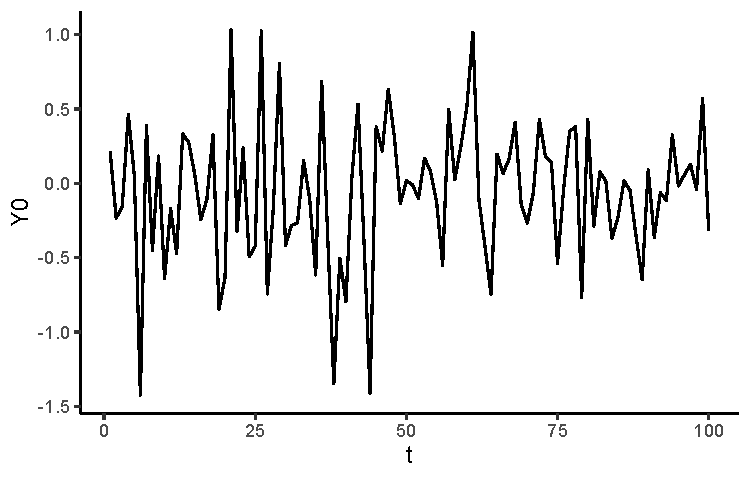
\includegraphics[width=0.5\linewidth]{figs_L1/stationary-1} \end{center}
\end{block}
\end{frame}

\begin{frame}{}
\protect\hypertarget{section}{}
\begin{block}{Example 2: Stationary process (correlated error)}
\protect\hypertarget{example-2-stationary-process-correlated-error}{}
\begin{itemize}
\item
  Data below were generated using \(\mu=0\) and errors that followed a
  first-order autoregressive \(\big(AR(1)\big)\) process:
  \(\epsilon_t = \phi\epsilon_{t-1} + Z_t\) and Specifically,
  \(Z_t \stackrel {iid} \sim \mathcal {N} (0,\ 0.46)\), for all \(t\).
\item
  \textbf{Notes on AR(1) processes}:

  \begin{enumerate}
  \item
    Errors \(\epsilon_t\) are identically distributed but not
    independent
  \item
    Must have \(|\phi| < 1\) for stationary process
  \item
    The higher the value of \(|\phi|\), the higher degree of correlation
    between responses from day to day
  \end{enumerate}
\end{itemize}
\end{block}
\end{frame}

\begin{frame}{}
\protect\hypertarget{section-1}{}
\begin{block}{Example 2: Stationary process (correlated error)}
\protect\hypertarget{example-2-stationary-process-correlated-error-1}{}
\begin{center}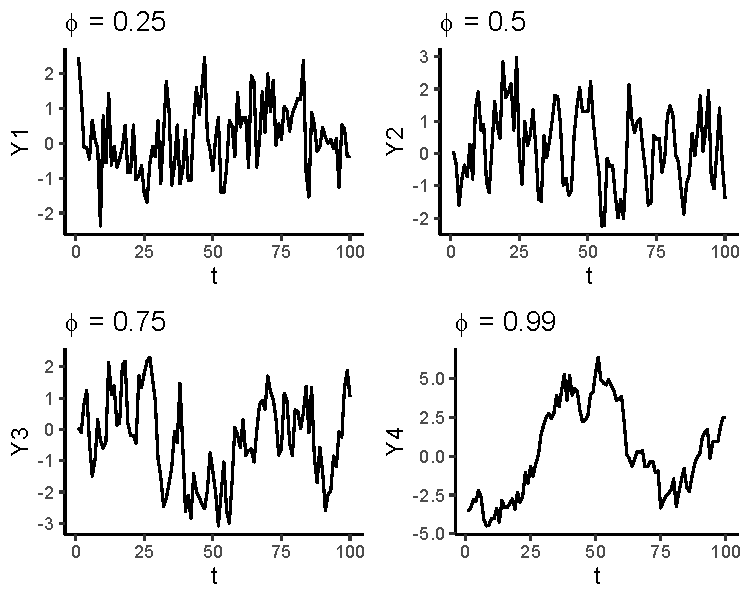
\includegraphics[width=0.9\linewidth]{figs_L1/AR1-1} \end{center}
\end{block}
\end{frame}

\begin{frame}{}
\protect\hypertarget{section-2}{}
\begin{block}{Example 3: Processes with trend and correlated errors}
\protect\hypertarget{example-3-processes-with-trend-and-correlated-errors}{}
\begin{itemize}
\item
  \(AR(1)\) process with linear time trend.
\item
  \(Y_t = \beta_0 + \beta_1t + \epsilon_t\), \(\beta_0 = 0\),
  \(\beta_1 = -0.05\), \(\epsilon_t \sim AR(1)\)\\
  (as in \textbf{Example 2}, last page, with \(\phi\ =\ 0.25\))
\end{itemize}

\begin{center}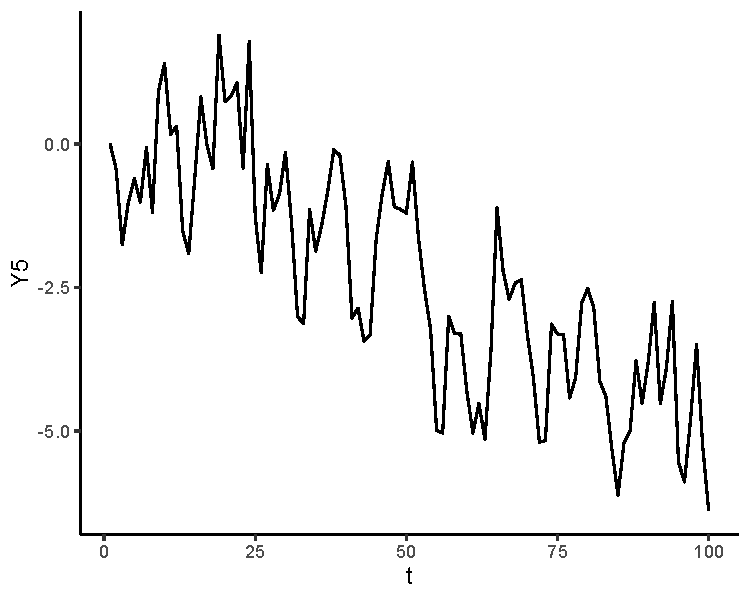
\includegraphics[width=0.5\linewidth]{figs_L1/linear time trend-1} \end{center}

\textbf{Random walks - see course notes (includes Example 5)}
\end{block}
\end{frame}

\hypertarget{longitudinal-data-types-and-examples}{%
\section{Longitudinal data types and
examples}\label{longitudinal-data-types-and-examples}}

\begin{frame}{}
\protect\hypertarget{section-3}{}
\begin{block}{Example 4: Retrospective observational studies}
\protect\hypertarget{example-4-retrospective-observational-studies}{}
\begin{itemize}
\item
  Longitudinal trajectories of pseudomonas (PA) in EPIC study

  \begin{itemize}
  \item
    1734 children enrolled in the EPIC observational study who were
    pseudomonas negative (PA-) for early pseudomonas infection control
    observational study (EPIC)
  \item
    Median followup time is 7.8 years (\(Q1 - Q3:\ 6.3 - 8.3\))
  \item
    One of the questions of interest was finding factors associated with
    progression of PA; A secondary outcome of interest: time to first
    pulmonary exacerbation in EPIC trial
  \end{itemize}
\end{itemize}

\begin{center}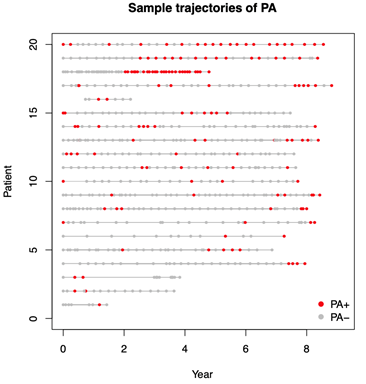
\includegraphics[width=0.5\linewidth]{figs_L1/L1-f1} \end{center}
\end{block}
\end{frame}

\begin{frame}{}
\protect\hypertarget{section-4}{}
\begin{block}{Example 5: Prospective observational studies}
\protect\hypertarget{example-5-prospective-observational-studies}{}
STEPPED-CARE randomized trial.

\begin{itemize}
\tightlist
\item
  A behavioral intervention was tested versus usual care in patients
  with lung or head and neck cancer.
\end{itemize}

\alert {*need some figures*}
\end{block}
\end{frame}

\begin{frame}{}
\protect\hypertarget{section-5}{}
\begin{block}{Example 6: Chronic fatigue syndrome study}
\protect\hypertarget{example-6-chronic-fatigue-syndrome-study}{}
Complement levels and Chronic fatigue syndrome (CFS) data (Sorensen et
al., 2003).

\begin{itemize}
\item
  Involved measuring complement split products (biological markers) over
  time.
\item
  In this case, groups involved those with or without CFS, and thus
  repeated measures only involved time.
\item
  A special covariance structure was used to model the repeated measures
  since measurement times were unequally spaced.
\end{itemize}
\end{block}
\end{frame}

\begin{frame}{}
\protect\hypertarget{section-6}{}
\begin{block}{Example 7: Growth curve data}
\protect\hypertarget{example-7-growth-curve-data}{}
\begin{itemize}
\item
  Graphs for height as a function of age for boys and girls aged 2 to 20
  years
\item
  Constructed in R after obtaining growth data from the
  \href{http://www.cdc.gov/}{CDC}. For more information, please see
  \href{http://www.cdc.gov/growthcharts/}{growcharts}.
\item
  These data show that girls approach their maximum height much more
  quickly than boys. The y-axis scales were made the same for easier
  comparison between graphs.
\item
  Each curve is a percentile estimate as a function of age. We could
  create confidence bands for each percentile curve.
\item
  If the curves are estimated using a lot of data, the widths of the
  bands should be narrow. Doctors look for dramatic changes between
  visits.
\item
  The curves here may not be representative of all populations (e.g.,
  differences due to race).
\end{itemize}
\end{block}
\end{frame}

\begin{frame}{}
\protect\hypertarget{section-7}{}
\begin{block}{Example 7: Growth curve data}
\protect\hypertarget{example-7-growth-curve-data-1}{}
\begin{center}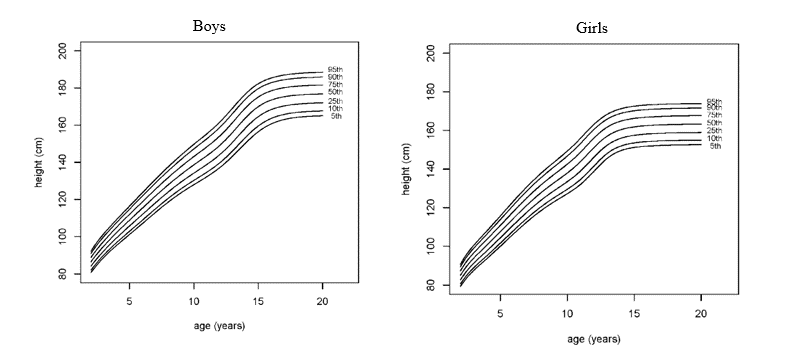
\includegraphics[width=1\linewidth]{figs_L1/L1-f2} \end{center}

\textbf{See course notes for more data examples}
\end{block}
\end{frame}

\begin{frame}{Formats for longitudinal data}
\protect\hypertarget{formats-for-longitudinal-data}{}
This section covers

\begin{itemize}
\item
  how to set up data for ``univariate'' versus ``multivariate'' analysis
\item
  types of variables and notation for variables in longitudinal data
  versus ``factorial'' data
\item
  \textbf{See course notes for more information}
\end{itemize}
\end{frame}

\begin{frame}{}
\protect\hypertarget{section-8}{}
\begin{block}{Example 8, 9, \& 10: Cluster data}
\protect\hypertarget{example-8-9-10-cluster-data}{}
\textbf{Example 8}: After an exercise challenge performed on 20
subjects, resting heart rates are monitored at 5 minute intervals for
one hour. How are data clustered?

\textbf{Example 9}: Families are selected to participate in a survey
regarding health insurance.\\
Each member of the family will be included in the study.

\textbf{Example 10}: arm length and leg length growth are measured for
subjects once a year for 10 years, and then modeled with a linear mixed
model.
\end{block}
\end{frame}

\hypertarget{simple-clusteredlongitudinal-analyses}{%
\section{Simple clustered/longitudinal
analyses}\label{simple-clusteredlongitudinal-analyses}}

\begin{frame}{What we've already done!}
\protect\hypertarget{what-weve-already-done}{}
\begin{itemize}
\item
  Experiments with pre-post measurements have 2 measurements on each
  subject over time. When there are only 2 measurements, the analysis
  simplifies when the difference is considered, as the analysis is
  reduced to one measurement per subject. Simple methods can then be
  used (e.g., paired t-test).
\item
  Longitudinal models can still be beneficial here! But we'll discuss
  that later. For now, we consider simplified models.
\item
  Let's take a closer look at the underlying models when we use a
  difference score or take the baseline-as-covariate approach.
\end{itemize}
\end{frame}

\begin{frame}{Change-score model and Baseline-as-covariate model}
\protect\hypertarget{change-score-model-and-baseline-as-covariate-model}{}
\begin{block}{Change-score model}
\protect\hypertarget{change-score-model}{}
\[
Y_{i1} = Score_{pre}; \ Y_{i2} = Score_{post} 
\] \vspace{-5mm} \[
\Delta_i = Y_{i1} - Y_{i2} = \beta_0 + \beta_1 x_i + \epsilon_i
\]
\end{block}

\begin{block}{Baseline-as-covariance model}
\protect\hypertarget{baseline-as-covariance-model}{}
\[
Y_{i2} = \beta_0 +\beta_1Y_{i1} + \beta_2 x_i + \epsilon_i
\]

We allow the slope of the baseline value to be anything (based on fit).
\end{block}

\begin{block}{Example for discussion: cholesterol data}
\protect\hypertarget{example-for-discussion-cholesterol-data}{}
Any other type of simple clustering, with 2 responses per cluster can be
analyzed similarly. (E.g., pairing by married couple, pairing by year of
measurement.)
\end{block}
\end{frame}

\hypertarget{usual-assumptions-for-longitudinal-models}{%
\section{Usual assumptions for longitudinal
models}\label{usual-assumptions-for-longitudinal-models}}

\begin{frame}{}
\protect\hypertarget{section-9}{}
\begin{itemize}
\item
  Assumption 1: Responses between subjects are independent.

  \begin{itemize}
  \item
    If there are clear violations to the assumption, and data are
    available, then a random term could be added to deal with this
    non-independence.
  \item
    For example, if a class is used for the sample, and there are
    several pairs of siblings in the class, a random term identifying
    family could be added to the model. (Lack of fit and lack of
    independence are related!)
  \end{itemize}
\item
  Assumption 2: There is a common covariance structure between all
  subjects, and the covariance parameters have the same value between
  subjects.

  \begin{itemize}
  \item
    This assumption is usually not tested. However, to properly estimate
    covariance parameters, several subjects are needed (just as data for
    several subjects are needed to estimate a common population mean).
  \item
    In some cases, homogeneous groups within the study may be identified
    (but heterogeneous between groups). With sufficient group sample
    sizes, group-specific covariance parameters can be put in the model
    and estimated.
  \end{itemize}
\end{itemize}
\end{frame}

\hypertarget{longitudinal-designs-and-power---an-initial-glimpse}{%
\section{Longitudinal designs and power - an initial
glimpse}\label{longitudinal-designs-and-power---an-initial-glimpse}}

\begin{frame}{Longitudinal designs and power - an initial glimpse}
\protect\hypertarget{longitudinal-designs-and-power---an-initial-glimpse-1}{}
\begin{itemize}
\item
  Consider an experiment designed to compare two treatments. Two common
  approaches:

  \begin{itemize}
  \item
    A1: Use independent samples (randomly assign some subjects one
    treatment, and some the other). For A1, we often use a 2-independent
    sample t-test
  \item
    A2: Have all subjects have one treatment and then have them all take
    the other (e.g., use a crossover design to eliminate confounding
    effects related to time). For A2, a paired t-test.
  \end{itemize}
\item
  A study/experiment involving changes within subjects (e.g., analyzed
  with a paired t-test) is often more powerful than a study using
  independent samples.
\end{itemize}
\end{frame}

\begin{frame}{}
\protect\hypertarget{section-10}{}
\begin{itemize}
\tightlist
\item
  The general formula for the variance for the difference in means
  suggests why this may be expected (when correlations between responses
  within subjects are positive):
\end{itemize}

\[
Var[\bar Y_1 - \bar Y_2] = Var[\bar Y_1] + Var[\bar Y_2] - 2Cov[\bar Y_1,\ \bar Y_2]
\]

\begin{itemize}
\item
  Often there are many factors not of interest that distinguish the two
  independent samples, while for the paired data, the difference in
  responses is due more to the treatment alone and not to other factors,
  since we're using the same subjects.
\item
  The same principle generalizing to multiple times and longitudinal
  data in general (e.g., air pollution study); subject serve as their
  own controls.
\item
  But paired/longitudinal designs may not always be better. In some
  cases a short cross-sectional study/experiment involving many subjects
  may be more feasible and cost-effective.
\end{itemize}
\end{frame}

\begin{frame}{Summary}
\protect\hypertarget{summary}{}
\begin{enumerate}
\item
  Why do we need special methods?
\item
  Discussed example datasets that are longitudinal
\item
  Discuss time series vs.~longitudinal; formats for longitudinal data
\item
  Assumptions for longitudinal models
\item
  Analyses of longitudinal data with two time points
\end{enumerate}
\end{frame}

\end{document}
